\documentclass[24pt,aspectratio=169]{beamer}
\graphicspath{{Images/}{./}} % Specifies where to look for included images (trailing slash required)
\usetheme{metropolis}

\usepackage[spanish]{babel} % Cargar el paquete babel con la opción spanish
\usepackage[utf8]{inputenc} % Asegurar la codificación UTF-8
\usepackage{appendixnumberbeamer}
\usepackage{booktabs}
\usepackage[scale=2]{ccicons}
\usepackage{pgfplots}
\usepackage{xcolor} % Cargar el paquete xcolor
\usepackage{xspace}
\usepackage[round]{natbib}
\usepackage{ragged2e}
\usepackage{bbding} %palomitas checkmark
\usepgfplotslibrary{dateplot}

\usepackage[ruled,vlined]{algorithm2e}
\usepackage{dirtree}
\usepackage{xcolor}

\usepackage{rotating}
\usepackage{tikz}

\usepackage{array} % needed for \arraybackslash
\usepackage{graphicx}
\usepackage{adjustbox} % for \adjincludegraphics

\usepackage{subcaption}
\usepackage{bibentry}
%\bibliographystyle{apalike}
\usepackage{chngcntr}
\usepackage{lipsum}% http://ctan.org/pkg/lipsum
\usepackage{hanging}% http://ctan.org/pkg/hanging

\usepackage{xcolor,colortbl}
\usepackage{multirow}

\usepackage{animate}
\usepackage{multicol}
\usepackage{tabularx,booktabs}
\usepackage{forloop}
\usepackage{ragged2e}

\usepackage{bbding} %palomitas checkmark
\usepackage{pifont}
\usepackage{lipsum,tabularx}

\usepackage{tikz}
\usetikzlibrary{arrows.meta, positioning, shapes.multipart}

\usepackage{tikz}
\usetikzlibrary{shapes,arrows}
\usepackage{amsmath,bm,times}

\usepackage{enumitem}

%\usepackage{circuitikz}
\usepackage{longtable}

\usepackage{progressbar}

\usepackage{pgfgantt}

\newcommand{\mx}[1]{\mathbf{\bm{#1}}} % Matrix command
\newcommand{\vc}[1]{\mathbf{\bm{#1}}} % Vector command

%\usepackage{annotate-equations}
\newcounter{loopcntr}

\definecolor{verde_cinves}{HTML}{009383} % Color de primer plano (foreground) de la barra de progreso
\definecolor{azulrey_cinves}{HTML}{005179} % Color de primer plano (foreground) de la barra de progreso
\definecolor{amarillo_cinves}{HTML}{FFDA72} % Color de primer plano (foreground) de la barra de progreso

\newcommand{\themename}{\textbf{\textsc{metropolis}}\xspace}

%separador titulo inicio
\setbeamercolor{title separator}{use=structure,fg=azulrey_cinves!50, bg=azulrey_cinves!10}

%barra que anuncia el nombre de la seccion
\setbeamercolor{progress bar in section page}{use=structure,fg=azulrey_cinves!100, bg=azulrey_cinves!10}

%barra de titulo en cada section page
\setbeamercolor{frametitle}{use=structure,fg=azulrey_cinves!5, bg=azulrey_cinves!100}

\title{\large{Estrategias para la exploración coordinada multi-VANT}}
%\subtitle{A modern beamer theme}
\author{Tesista: Luis Alberto Ballado Aradias\\[\baselineskip]
  \small{{Asesores:} 
    \and\\Dr. José Gabriel Ramírez-Torres
    \and\\Dr. Eduardo Rodriguez-Tello\\ }}
\date{\today}
\institute{Centro de Investigación y de Estudios Avanzados - Unidad Tamaulipas}
\titlegraphic{\hfill
\includegraphics[height=1.5cm]{cinvestav_negro}}

\newcommand{\rpt}[2][1]{%
  \forloop{loopcntr}{0}{\value{loopcntr}<#1}{#2}%
}

\newcommand{\on}[1][1]{
  \forloop{loopcntr}{0}{\value{loopcntr}<#1}{&\cellcolor{lightgray}}
}
\newcommand{\onok}[1][1]{
  \forloop{loopcntr}{0}{\value{loopcntr}<#1}{&\cellcolor{green}}
}
\newcommand{\ondelay}[1][1]{
  \forloop{loopcntr}{0}{\value{loopcntr}<#1}{&\cellcolor{red}}
}
\newcommand{\off}[1][1]{
  \forloop{loopcntr}{0}{\value{loopcntr}<#1}{&\cellcolor{white}}
}

\addtolength{\textheight}{90pt}

\newcommand{\I}{\mathbb{I}}
\newcommand{\K}{\mathbb{K}}
\newcommand{\N}{\mathbb{N}}
\newcommand{\Q}{\mathbb{Q}}
\newcommand{\R}{\mathbb{R}}
\newcommand{\Z}{\mathbb{Z}}

\newcommand{\specialcell}[2][c]{%
  \begin{tabular}[#1]{@{}c@{}}#2\end{tabular}}

% Definir comandos para checkmark y cross
\newcommand{\cmark}{{\color{green}\ding{51}}} % Checkmark en verde
\newcommand{\xmark}{{\color{red}\ding{55}}}   % Cross en rojo

%Used to draw gantt charts, which I will use for the calendar.
%Let's define some awesome new ganttchart elements:
\newganttchartelement{orangebar}{
    orangebar/.style={
        inner sep=0pt,
        draw=red!66!black,
        very thick,
        top color=white,
        bottom color=orange!80
    },
    orangebar label font=\slshape,
    orangebar left shift=.1,
    orangebar right shift=-.1
}

\newganttchartelement{bluebar}{
    bluebar/.style={
        inner sep=0pt,
        draw=purple!44!black,
        very thick,
        top color=white,
        bottom color=blue!80
    },
    bluebar label font=\slshape,
    bluebar left shift=.1,
    bluebar right shift=-.1
}

\newganttchartelement{greenbar}{
    greenbar/.style={
        inner sep=0pt,
        draw=green!50!black,
        very thick,
        top color=white,
        bottom color=green!80
    },
    greenbar label font=\slshape,
    greenbar left shift=.1,
    greenbar right shift=-.1
}

\begin{document}

\maketitle

\begin{frame}{Contenido}
  \setbeamertemplate{section in toc}[sections numbered]
  \tableofcontents[hideallsubsections]
\end{frame}

\section{Introducción}

\begin{frame}[fragile]{Antecedentes}
  \bigskip % Vertical whitespace
  \centering
  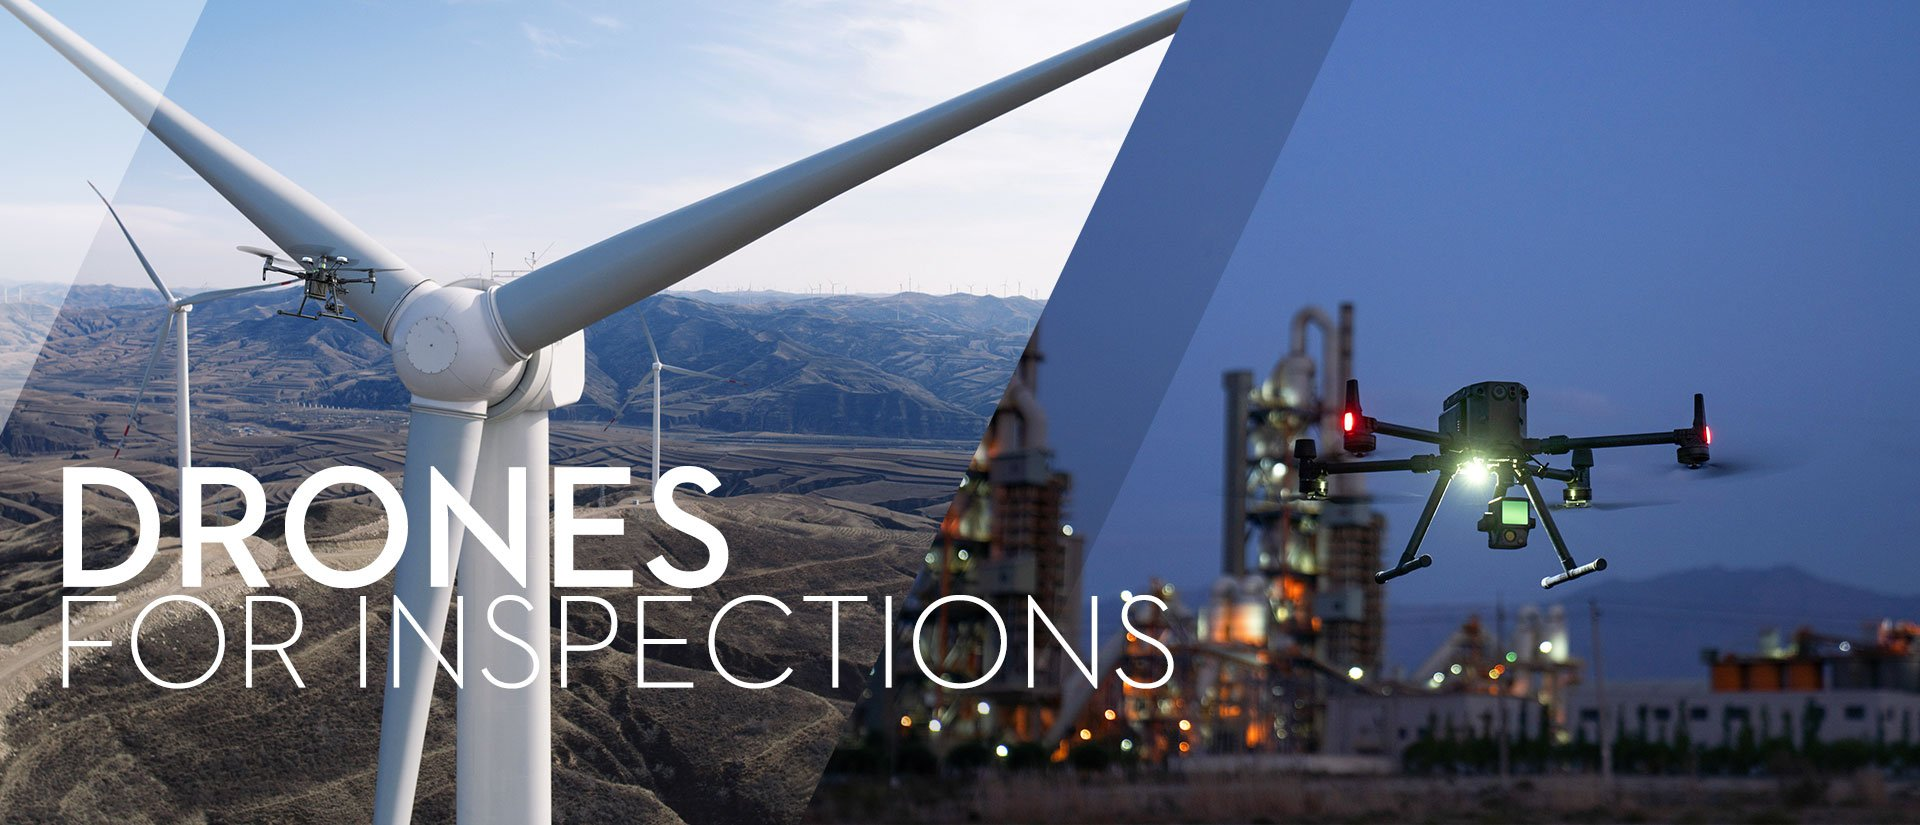
\includegraphics[width=0.45\textwidth,height=0.35\textheight]{DJI_B1}$^\dag$
  \hfil
  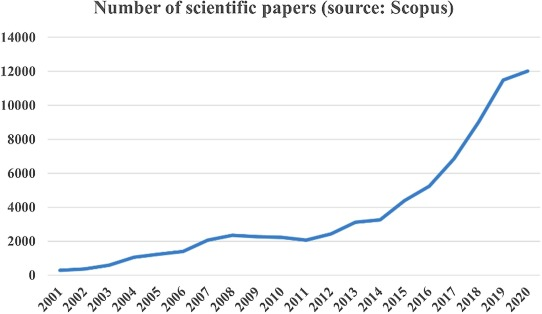
\includegraphics[width=0.45\textwidth,height=0.35\textheight]{survey_chart.jpg}\footnotemark
  %\vspace{1pt}\\
  
  \begin{itemize}
  \item \textbf{UAV} {\tiny(\textit{Vehículo Aéreo No Tripulado - VANT})}  $\implies$ \textbf{UAS} {\tiny(\textit{Sistemas Aéreos No Tripulado - SANT})}
  \item \textbf{Aplicaciones} en lugares inaccesibles o peligrosos.
  \item \textbf{Múltiples VANT} pueden aumentar la confianza del sistema.
  \item \textbf{Limitaciones} en carga, procesamiento y batería \small{influyen en el tiempo de vuelo.}
  \end{itemize}
  
  \tiny{
    \footnotetext{UAV in the advent of the twenties: Where we stand and what is next [\cite{Nex2022}]}
  }
\end{frame}

\begin{frame}[fragile]{Antecedentes}
  
  %\centering
  Principales preguntas que un robot autónomo debe responder \footnotemark\\
  \begin{itemize}
  \item ¿Dónde estoy? $\implies$ Localización 
  \item ¿A dónde voy? $\implies$ Cognición
  \item ¿Cómo llego hasta ahí? $\implies$ Planificación de trayectoria
  \end{itemize}
  %\pause
  %\bigskip % Vertical whitespace
  Para resolver estas preguntas, el robot debe:\\
  \begin{itemize}
  \item Tener un modelo del ambiente (dado, o autónomamente construido)
  \item Localizarse dentro del ambiente
  \item Planear y ejecutar sus movimientos
  \end{itemize}

  \footnotetext{Visual map making for a mobile robot [\cite{1087348}]}
  
\end{frame}

\begin{frame}{Antecedentes}
  \centering
  \textbf{Arquitectura de un robot móvil}
  \bigskip % Vertical whitespace
  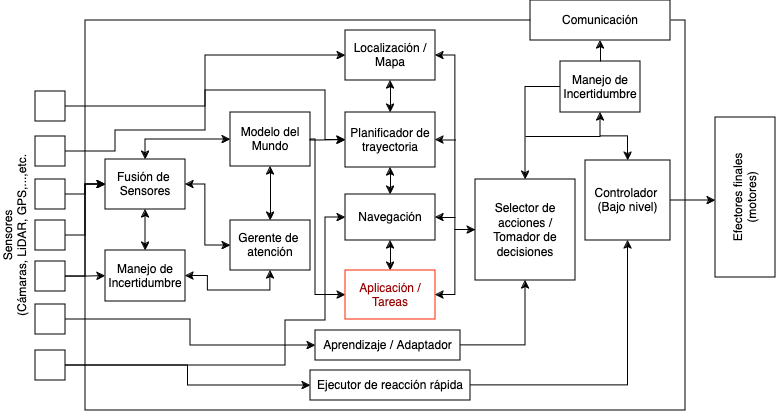
\includegraphics[width=11cm]{arquitectura_robots}\\
\end{frame}

\begin{frame}{Antecedentes}

  %Exploración es una tarea fundamental en robots autónomos.\\
  %El objetivo es crear un mapa de un ambiente desconocido.\\
  %\bigskip % Vertical whitespace
  \centering
  \bigskip % Vertical whitespace
  
\includegraphics[width=9cm]{exploracion}\\
  
  \begin{itemize}
  \item \textbf{Sensar}
  \item \textbf{Creación Mapa} 
  \item \textbf{Localización en Mapa}
  \item \textbf{\textcolor{blue}{Exploración}} (Aumentar la base de conocimiento del mapa)
  \item \textbf{\textcolor{blue}{Planificación trayectoria}} (Trayectorias hacia nuevas fronteras) 
  \item \textbf{Control} (Toma de decisiones y ejecución de trayectorias)
  \end{itemize}
  
  \alert{- El ciclo se repite hasta completar la exploración -}

\end{frame}

\begin{frame}[fragile]{Motivación del proyecto}
  %https://ccc.inaoep.mx/~emorales/Papers/2009/eduardo.pdf
  %https://www.mdpi.com/2504-446X/7/1/62
  %Hablar de los usos e importancia del trabajo .. de la exploracion .. de la importancia de investigacion en robotica para el pais.
  %El potencial del uso de UAVs en tareas de búsqueda y rescate, inspección, mapeo, vigilancia, entre otras, es de gran interés a explorar, debido a las habilidades de vuelo que presentan en favor de la realización de estas tareas, y en especial situaciones que podrían poner en riesgo a personas.\\
  %Enviar personal de rescate dentro de un edificio parcialmente colapsado por un terremoto en busca de sobrevivientes, es poner a más personas en un gran riesgo, pues no se sabe qué es lo que les espera en el interior del edificio; esto limita la capacidad de tomar buenas decisiones acerca de si es seguro seguir cierto camino.
  \begin{figure}[ht!]
    \centering
    \begin{minipage}{0.48\textwidth}
      \centering
      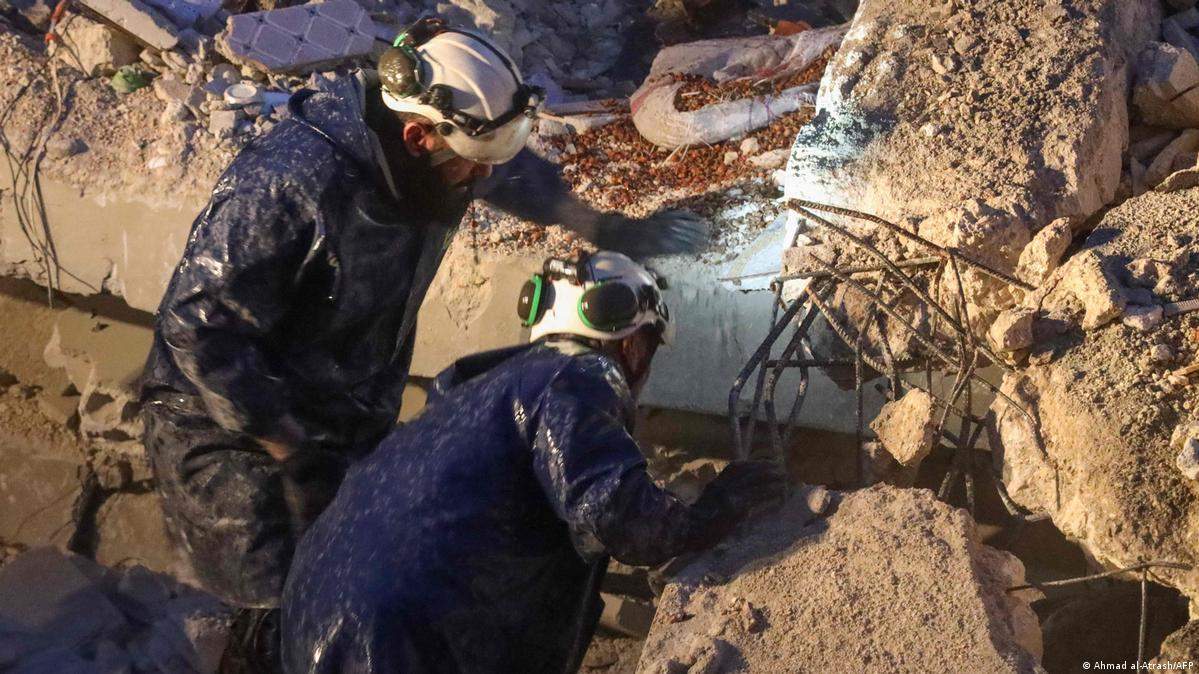
\includegraphics[width=\linewidth,height=3.5cm]{turquia1.jpg} % BUSQUEDA Y RESCATE
      %\caption{Primera Imagen}
    \end{minipage}\hfill
    \begin{minipage}{0.48\textwidth}
      \centering
      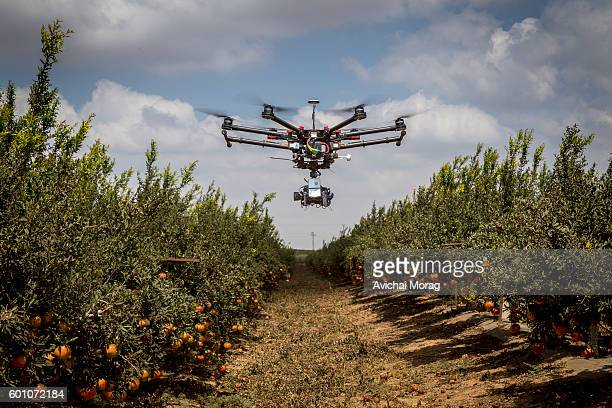
\includegraphics[width=\linewidth,height=3.5cm]{drone_agriculture.jpg} % INSPECCION Y SEGURIDAD
      %\caption{Segunda Imagen}
    \end{minipage}
    \vspace{-0.2cm} % Espacio vertical entre imágenes
    \begin{minipage}{0.48\textwidth}
      \centering
      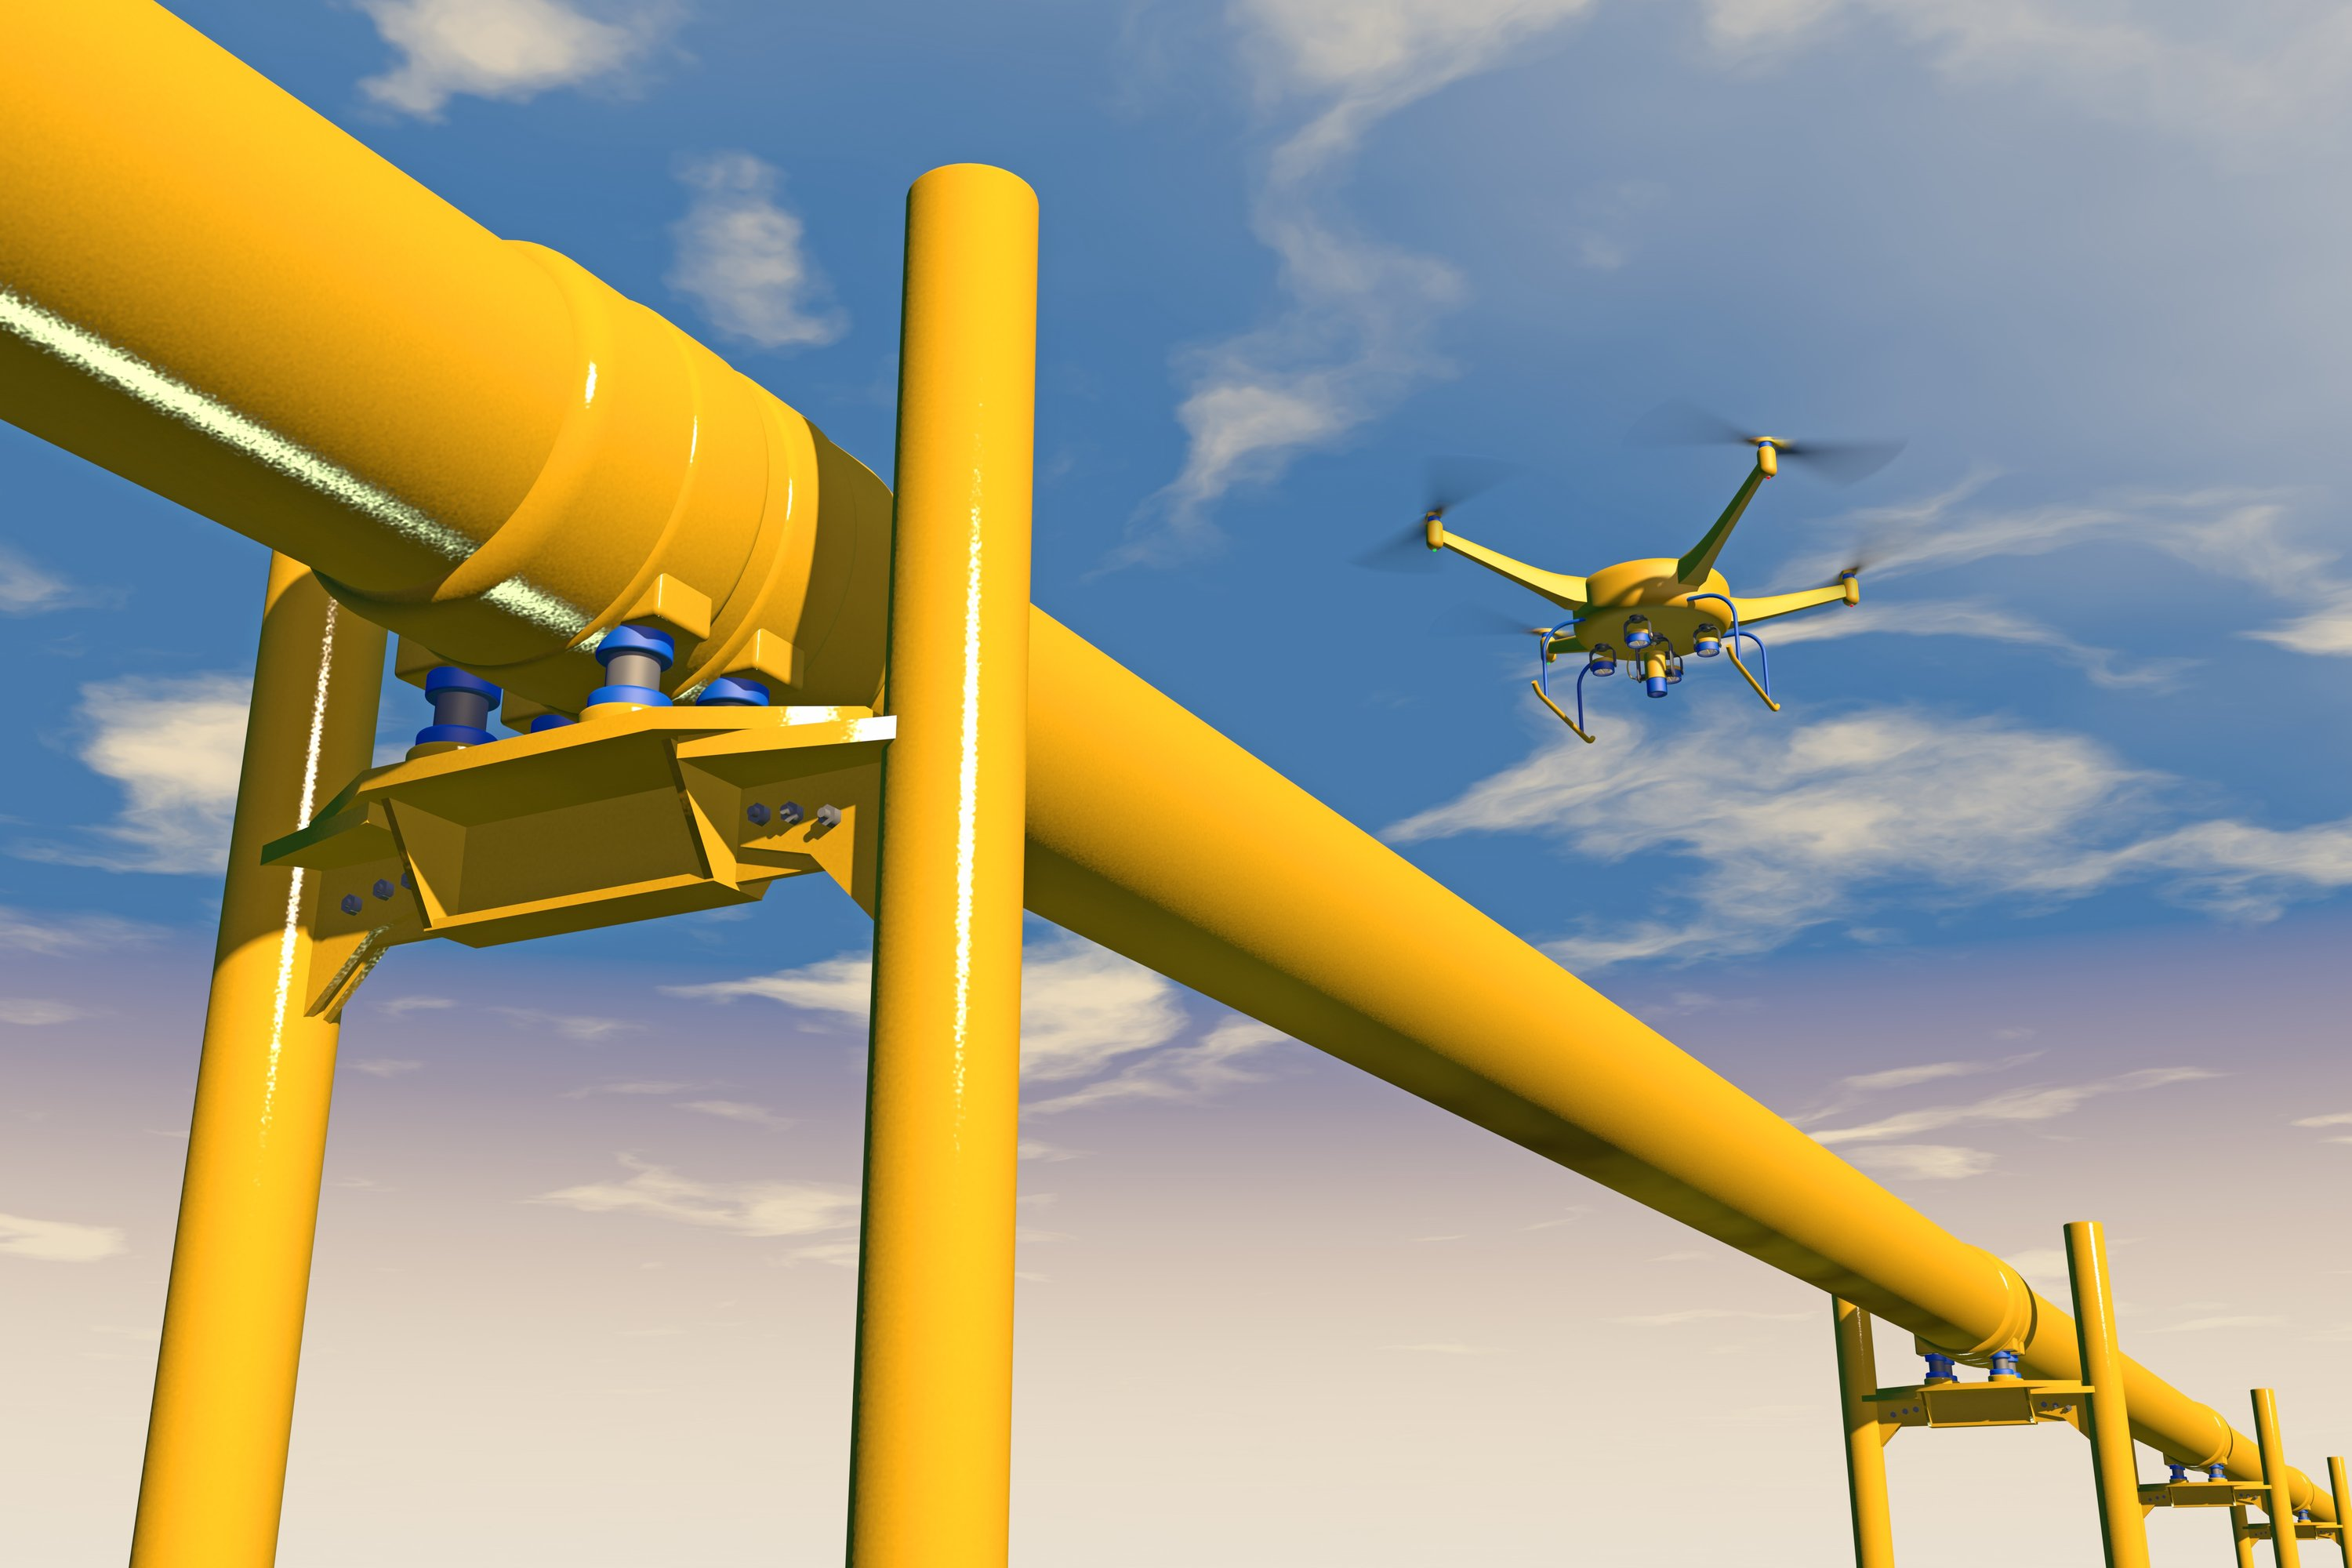
\includegraphics[width=\linewidth,height=3.5cm]{pipe_drone.jpg} % DRONES EN CIUDADES CON GPS DENY
      %\caption{Tercera Imagen}
    \end{minipage}\hfill
    \begin{minipage}{0.48\textwidth}
      \centering
      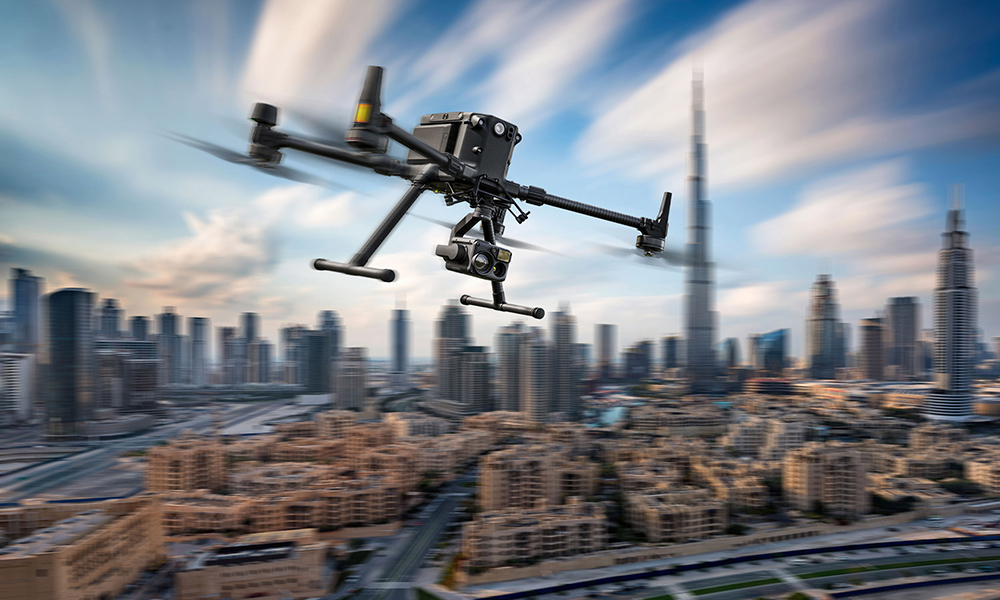
\includegraphics[width=\linewidth,height=3.5cm]{drone_city.jpg} % 
      %\caption{Cuarta Imagen}
    \end{minipage}
  \end{figure}
\end{frame}

\section{Planteamiento del problema}

\begin{frame}[fragile]{Planteamiento del problema}
  \vspace{1mm}
  \centering
  %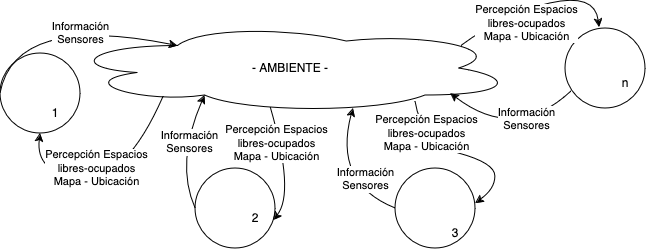
\includegraphics[width=9.5cm]{problema}\\
  \justifying
  \footnotesize Dado un volumen de interés desconocido en un espacio cerrado que se desea explorar denotado como $\mathcal{W}$, tal que $\mathcal{W} \subset \mathbb{R}^{3}$.\\
%el volumen se discretiza en un mapa de ocupación M consistente en voxeles cúbicos $m \exists M$ con una longitud de arista r.
  \begin{itemize}
  \item El volumen se discretiza usando unidades cúbicas tridimencionales (voxel) $v_{libre}$, $v_{ocup}$, $v_{desc}$.
    %La representación del volumen a explorar se obtiene dividiendo el volumen de interés en unidades cúbicas tridimencionales (voxel) que puede tomar los valores de libre $v_{libre}$, ocupado $v_{ocup}$ y desconocido $v_{desc}$ con lecturas a partir de los valores de una cámara RGB-D basada en un modelo de ocupación probabilístico.\\
  \item Un conjunto de VANTS con una cámara RGB-D embarcadas denotado como $\mathcal{V} = \{\mathcal{V}_{1},\mathcal{V}_{2},\mathcal{V}_{3},...,\mathcal{V}_{n}\}$, comenzando cada uno en un estado inicial conocido $q = \{q_{1},q_{2},q_{3},...,q_{n}\}$, y terminando en una configuración que maximice la construcción de un mapa.\\
  \end{itemize}

  \begin{center}
    \textcolor{blue}{Coordinar el conjunto de VANTs para reducir el tiempo total de exploración.}
  \end{center}
  
  \begin{multicols}{2}
    \begin{itemize}[label={}]
    \item \cmark { }Comprensión dinámica del VANT, VIO, planificador global
    \item \cmark { }Implementación planificador local en $\mathbb{R}^{3}$
    \item \cmark { }Implementación estrategia de coordinación
    \end{itemize}
    
    
    \begin{itemize}[label={}]
    \item \xmark { }Perturbaciones (vientos, lluvia, iluminación, ...etc.)
    \item \xmark { }Problemas de batería
    \item \xmark { }Interferencias de comunicación
    \end{itemize}
  \end{multicols}
  
  %Crear una Coordinar un conjunto de vehiculos aereos no tripulados
  %Explorar un volumen desconocido tal que $V \subset R^{3}$ con un conjunto de robots aéreos autónomos $R ={R_1,R_2,...,R_n}$, siendo n la cardinalidad del conjunto de robots aéreos. Cada robot cuenta con capacidades de generar una representación del medio ambiente, localizarse y generar trayectorias que minimicen la incertidumbre de la localización y el mapeo, evaluada a través de una métrica sobre la creencia probabilística de la pose del robot y la posición de los puntos de referencia. El problema de exploración puede formularse globalmente como el de partir de una configuración inicial libre de colisiones y derivar puntos de vista que cubran el volumen previamente desconocido, determinando qué partes del espacio inicialmente inexplorado están libres o ocupadas. Para este proceso, el volumen se discretiza en un mapa de ocupación M consistente en voxeles cúbicos $m \exists M$ con una longitud de arista r. La operación está sujeta a las restricciones dinámicas del vehículo y a las limitaciones del sistema de sensores. Dado que las capacidades perceptivas de la mayoría de los sensores terminan en las superficies, los espacios huecos o bolsillos estrechos a veces pueden permanecer inexplorados, lo que lleva a un volumen residual.
\end{frame}

\begin{frame}{Hipótesis y preguntas de investigación}
  
  \begin{block}{Hipótesis}
    \vspace{1mm}
    \small Una estrategia que coordine y asigne tareas de exploración para múltiples VANTS de manera descentralizada, en combinación con una arquitectura de software diseñada para resolver problemas de localización, gestión de mapas y planificación de rutas, mejorará la eficiencia y cobertura de la exploración en interiores de un entorno desconocido.
  \end{block}
  %\pause
  %\textcolor{blue}{Preguntas de investigación}
  \begin{block}{Preguntas de investigación}
    \small{
      \begin{enumerate}
      \item ¿Qué características de la dinámica del VANT son clave para generar trayectorias suaves y continuas?
      \item ¿Podría un planificador de trayectorias que aproveche las regiones libres de obstáculos acelerar los desplazamientos de los VANTs y, consecuentemente, reducir los tiempos de exploración?
      \item ¿Qué mecanismos de coordinación existen dentro de la literatura que podrían ayudar en resolver el problema de exploración multi-VANT?
      \end{enumerate}
    }
  \end{block}
\end{frame}

\begin{frame}{Objetivos}
  
  \begin{block}{Objetivo General}
    %Desarrollar una estrategia de exploración descentralizada que permita resolver los problemas de coordinación para múltiples VANTS en ambientes desconocidos.
    %Desarrollar una estrategia de exploración descentralizada que integre técnicas de percepción y algoritmos de decisión para mejorar la autonomía de múltiples VANTs en la exploración de interiores.
    \vspace{1mm}
    Desarrollar una estrategia de exploración descentralizada que permita resolver los problemas de coordinación para múltiples VANTS en ambientes desconocidos.
  \end{block}
  %\pause
  \bigskip
  \begin{block}{Objetivos Particulares}
    %\vspace{2mm}
    \begin{enumerate}
    \item Desarrollar una arquitectura de software que resuelva los problemas de autonomía para un VANT (localización, manejo de mapas y planificación de trayectorias).
    \item Implementar un mecanismo de coordinación descentralizado que asigne tareas de exploración.
    \item Realizar pruebas y simulaciones de la solución propuesta en diversos entornos, analizando la relación tiempo de exploración y cobertura del área de interés.
    \end{enumerate}
  \end{block}
\end{frame}

\begin{frame}{Estado del arte}
  \centering
  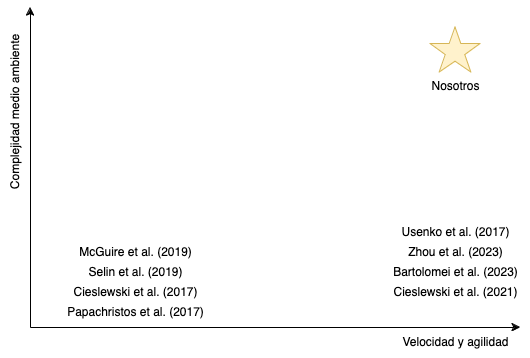
\includegraphics[width=10cm, height=6cm]{soa}
\end{frame}


\begin{frame}{Métodologia}
  \centering
  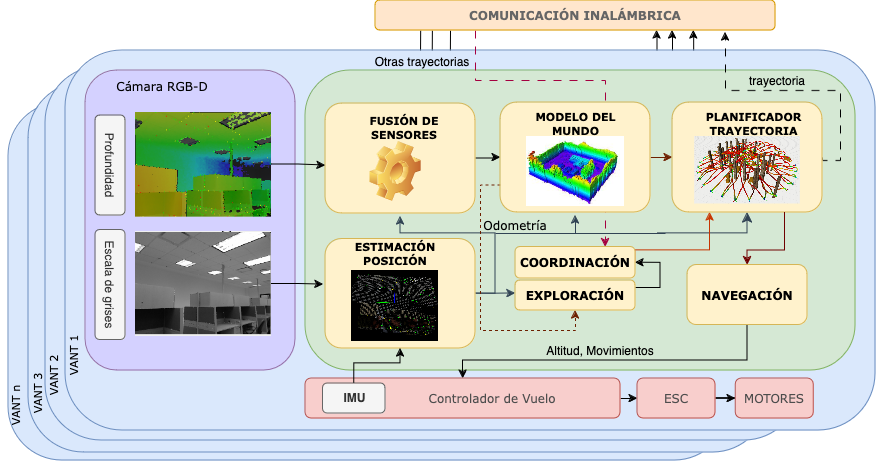
\includegraphics[width=10cm, height=6cm]{arquitectura}
\end{frame}

\begin{frame}{Avance}
  \bigskip % Vertical whitespace
  \centering
  \animategraphics[width=0.45\textwidth,height=0.45\textheight]{10}{ros_map_1/ros_map-}{0}{300}
  \hfil
  \animategraphics[width=0.45\textwidth,height=0.45\textheight]{10}{ros_map_2/ros_map-}{0}{239}
  \vspace{2pt}\\
  \textcolor{blue}{1 VANT}
  \hfil
  \textcolor{blue}{2 VANT}
\end{frame}


\section{Plan de cierre del trabajo}

\begin{frame}{}
  \bigskip % Vertical whitespace
  \tiny
  %\hspace{0.0cm}
  \begin{minipage}{5cm}
    \noindent\begin{tabular}{|p{0.8\textwidth}*{16}{|p{0.040\textwidth}}|}
    % The top line
    %\diagbox[width=12.5em]{Actividades}{Cuatrimestres}
    \hline
    & \multicolumn{4}{c|}{\color{teal!80}\textbf{Cuatrimestre 4}} 
    & \multicolumn{4}{c|}{\color{teal!80}\textbf{Cuatrimestre 5}} 
    & \multicolumn{4}{c|}{\color{teal!80}\textbf{Cuatrimestre 6}}
    & \multicolumn{4}{c|}{\textbf{Cuatrimestre Extra}}\\
    \hline
    % The second line, with its five years of four quarters
    %\textcolor{black}{\textbf{Etapas}}
    \rpt[4]{& 1 & 2 & 3 & 4} \\
    \hline
    \rowcolor{teal!40}{\textbf{Etapa 1}}\\
    % using the on macro to fill in twenty cells as `on'
    %\specialcell{Actividad 1\\espacio}        \on[0] \off[12] \\
    %Actividad 1    \on[0] \off[12]\\
    \hline
    \rowcolor{teal!15}{\textbf{E1.A1.} Revisi\'{o}n literatura relevante}
    %en exploraci\'{o}n multi-VANT, estrategias de exploraci\'{o}n, algoritmos de coordinaci\'{o}n y evaci\'{o}n de obst\'{a}culos
    \onok[9] \on[7]\\
    \hline
    %\textbf{E1.A2.} Evaluaci\'{o}n de aptitudes\footnote{Evaluaci\'{o}n a partir de los nuevos trabajos}     \on[12] \\
    %\hline
    \rowcolor{teal!15}{\textbf{E1.A2.} Selecci\'{o}n de algoritmos} \onok[2] \off[10] \\
    \hline
    \rowcolor{teal!15}{\textbf{E1.A3.} Dise\~{n}o de la AS\footnote{\tiny arquitectura de software}}
    \off[1] \onok[3] \on[0] \off[12] \\
    \hline
    \rowcolor{teal!15}{\textbf{E1.A4.} Documentaci\'{o}n Etapa 1}
    \onok[4] \on[0]  \off[12] \\
    \hline
    \rowcolor{teal!15}{\textbf{E1.A5.} Revisi\'{o}n de tesis Etapa 1}
    \off[3] \onok[1]  \off[12] \\
    \hline
    % using the on macro followed by the off macro
    \rowcolor{teal!40}{\textbf{Etapa 2}}\\
    \hline
    \rowcolor{teal!15}{\textbf{E2.A1.} Selecci\'{o}n Simulador}
    \onok[1]  \off[15] \\
    \hline
    \textbf{E2.A2.} Visualizaci\'{o}n de datos
    \off[1] \onok[2] \ondelay[6]  \off[7] \\
    \hline
    \textbf{E2.A3.} Control de desplazamientos
    \off[2] \onok[2] \ondelay[6] \off[6] \\
    \hline
    \textbf{E2.A4.} Desarrollo de AE \footnote{\tiny algoritmo de exploración}
    \off[3] \onok[2] \ondelay[5] \off[6] \\
    \hline
    %\rowcolor{teal!15}{\textbf{E2.A5.} Implementaci\'{o}n y simulaci\'{o}n}
    %\off[3] \onok[2] \ondelay[2] \off[5] \\
    %\hline
    %\textbf{E2.A6.} Simulaci\'{o}n un solo VANT
    %\off[4] \on[1] \off[7] \\
    %\hline
    \textbf{E2.A5.} Desarrollo de coordinaci\'{o}n
    \off[4] \on[3] \ondelay[4] \off[5] \\
    \hline
    \rowcolor{teal!15}{\textbf{E2.A6.} Implementaci\'{o}n y simulaci\'{o}n}
    \off[3] \onok[5] \ondelay[3] \off[5] \\
    \hline
    %\textbf{E2.A9.} Simulaci\'{o}n multi-VANT
    %\off[6] \on[1] \off[5] \\
    %\hline
    \rowcolor{teal!15}{\textbf{E2.A7.} Documentaci\'{o}n Etapa 2}
    \off[4] \onok[4] \off[8] \\
    \hline
    \rowcolor{teal!15}{\textbf{E2.A8.} Revisi\'{o}n de tesis Etapa 2}
    \off[7] \onok[1] \off[8] \\
    \hline
    \rowcolor{black!5}{\textbf{Etapa 3}}\\
    \hline
    \textbf{E3.A1.} Experimentaci\'{o}n de soluci\'{o}n
    \off[10]  \on[2] \off[4] \\
    \hline
    \textbf{E3.A2.} Recopilaci\'{o}n resultados
    \off[11]  \on[1] \off[4] \\
    \hline
    \textbf{E3.A3.} Documentaci\'{o}n Etapa 3
    \off[9] \on[3] \off[4] \\
    \hline
    \textbf{E3.A4.} Revisi\'{o}n de tesis
    \off[11] \on[3] \off[2]\\
    \hline
    \textbf{E3.A5.} Divulgaci\'{o}n
    \off[12]  \on[3] \off[1]\\
    \hline
    \textbf{E3.A6.} Proceso de titulaci\'{o}n
    \off[14] \on \off[1]\\
    \hline
    \end{tabular}
  \end{minipage}
\end{frame}

\begin{frame}{Semanas}
  \bigskip % Vertical whitespace
  \tiny
  %\hspace{0.0cm}
  \begin{minipage}{5cm}
    \noindent\begin{tabular}{|p{0.8\textwidth}*{16}{|p{0.020\textwidth}}|}
    % The top line
    %\diagbox[width=12.5em]{Actividades}{Cuatrimestres}
    \hline
    & \multicolumn{4}{c|}{\color{teal!80}\textbf{MAYO}} 
    & \multicolumn{4}{c|}{\textbf{JUNIO}} 
    & \multicolumn{4}{c|}{\textbf{JULIO}}
    & \multicolumn{4}{c|}{\textbf{AGOSTO}}\\
    \hline
    % The second line, with its five years of four quarters
    %\textcolor{black}{\textbf{Etapas}}
    \rpt[4]{& 1 & 2 & 3 & 4} \\
    \hline
    \rowcolor{teal!40}{\textbf{Visualización de datos}}\\
    \hline
    \textbf{A1.} Manejo estructura del mapa
    \off[1] \onok[2] \ondelay[6]  \off[7] \\
    \hline
    \textbf{A2.} Comprensión del FOV aplicado dentro del simulador
    \off[2] \onok[2] \ondelay[6] \off[6] \\
    \hline
    \textbf{A3.} Trazabilidad de la trayectoria
    \off[3] \onok[2] \ondelay[5] \off[6] \\
    \hline
    \textbf{A4.} Manejo de los mensajes en ROS
    \off[4] \on[3] \ondelay[4] \off[5] \\
    \hline
    \rowcolor{teal!15}{\textbf{A5.} Manejo de los tópicos en ROS}
    \off[3] \onok[5] \ondelay[3] \off[5] \\
    \hline
    \rowcolor{black!5}{\textbf{Etapa 3}}\\
    \hline
    \textbf{E3.A1.} Experimentaci\'{o}n de soluci\'{o}n
    \off[10]  \on[2] \off[4] \\
    \hline
    \textbf{E3.A2.} Recopilaci\'{o}n resultados
    \off[11]  \on[1] \off[4] \\
    \hline
    \textbf{E3.A3.} Documentaci\'{o}n Etapa 3
    \off[9] \on[3] \off[4] \\
    \hline
    \textbf{E3.A4.} Revisi\'{o}n de tesis
    \off[11] \on[3] \off[2]\\
    \hline
    \textbf{E3.A5.} Divulgaci\'{o}n
    \off[12]  \on[3] \off[1]\\
    \hline
    \textbf{E3.A6.} Proceso de titulaci\'{o}n
    \off[14] \on \off[1]\\
    \hline
    \end{tabular}
  \end{minipage}

  \begin{table}[h!]
    \centering
    \begin{tabular}{|m{1cm}|m{5cm}|m{5cm}|}
      \hline
      \textbf{Actividad} & \textbf{Producto} & \textbf{Incidencia} \\
      \hline
      A1 & 20 empleados capacitados & Mejora la interacción con los clientes, aumentando su satisfacción. \\
      \hline
      A2 & Sistema en funcionamiento 100\% & Permite resolución rápida y efectiva de quejas, reduciendo la insatisfacción. \\
      \hline
      A3 & Datos de encuestas y análisis d & Proporciona retroalimentación continua para mejorar el servicio. \\
      \hline
    \end{tabular}
    \caption{Tabla de actividades, productos e incidencia}
    \label{tab:actividad_producto_incidencia}
  \end{table}
\end{frame}

%TODO
%\begin{frame}{Gantt}
%\begin{minipage}{3cm}
%\tiny{
%\begin{ganttchart}[
%hgrid style/.style={black, dotted},
%vgrid={*5{black,dotted}, *1{white, dotted}, *1{black, dashed}},
%x unit=3mm,
%y unit chart=9mm,
%y unit title=12mm,
%time slot format=isodate,
%group label font=\bfseries \Large,
%link/.style={->, thick}
%]{2024-05-06}{2024-08-23}
%\gantttitlecalendar{year, month=name, week}\\
%\ganttgroup[
%group/.append style={fill=orange}
%]{\small Etapa 2}{2024-05-06}{2024-07-26}\\ [grid]
%\ganttorangebar[
%name=VIS
%]{Visualización Datos}{2024-05-06}{2024-05-15}\\ [grid]
%\ganttorangebar[
%name=FOVSim
%]{Comprension FOV Simulador}{2024-05-15}{2024-05-20}\\ [grid]
%\ganttorangebar[
%name=Trazabilidad
%]{Trazabilidad}{2024-05-20}{2024-05-22}
%\ganttlinkedorangebar{}{2024-05-06}{2024-05-15}
%\ganttlinkedorangebar{}{2024-05-15}{2024-05-22}
%\ganttlinkedorangebar{}{2014-10-17}{2014-10-17}
%\ganttlinkedorangebar[name=FMEend]{}{2014-10-21}{2014-10-24}
%\ganttlinkedorangebar{}{2014-10-28}{2014-10-31}\\ [grid]
%\ganttorangebar[name=Manual]{Manual}{2014-10-30}{2014-10-31}
%\ganttlinkedorangebar{}{2014-11-4}{2014-11-7} \ganttnewline[thick, black]
%\ganttgroup[
%group/.append style={fill=green}
%]{KLIP Manager}{2014-11-3}{2014-11-9}
%\ganttgroup[
%group/.append style={fill=green}
%]{}{2014-11-17}{2014-11-23}\\ [grid]
%\ganttgreenbar{Manual}{2014-11-4}{2014-11-7}
%\ganttlinkedgreenbar{}{2014-11-18}{2014-11-19}
%%Implementing links
%\ganttlink[link mid=0.75]{Documentation}{FME}
%\ganttlink{FMETutorial}{FME}
%\end{ganttchart}
%}
%\end{minipage}
%\end{frame}

%\begin{frame}{Ejemplo}
%\begin{table}
%\begin{tabular}{|l|c|c|}
%foo & bar & 
%\progressbar[linecolor=blue, filledcolor=green]{0.6}\llap{\raisebox{1.5pt}{\tiny$60\%$}\hspace{0.8cm}}  \\
%foo & bar & 
%\progressbar[linecolor=blue, filledcolor=green]{0.6}%
%\begin{picture}(0,0)
%\put(-35,1.5) {\tiny$60\%$}
%\end{picture}
%\end{tabular}
%\end{table}
%\end{frame}

\begin{frame}[standout]
  ¿Preguntas?
\end{frame}

\appendix

\section{Apéndice}

\begin{frame}{Robot autónomo}
  \centering
  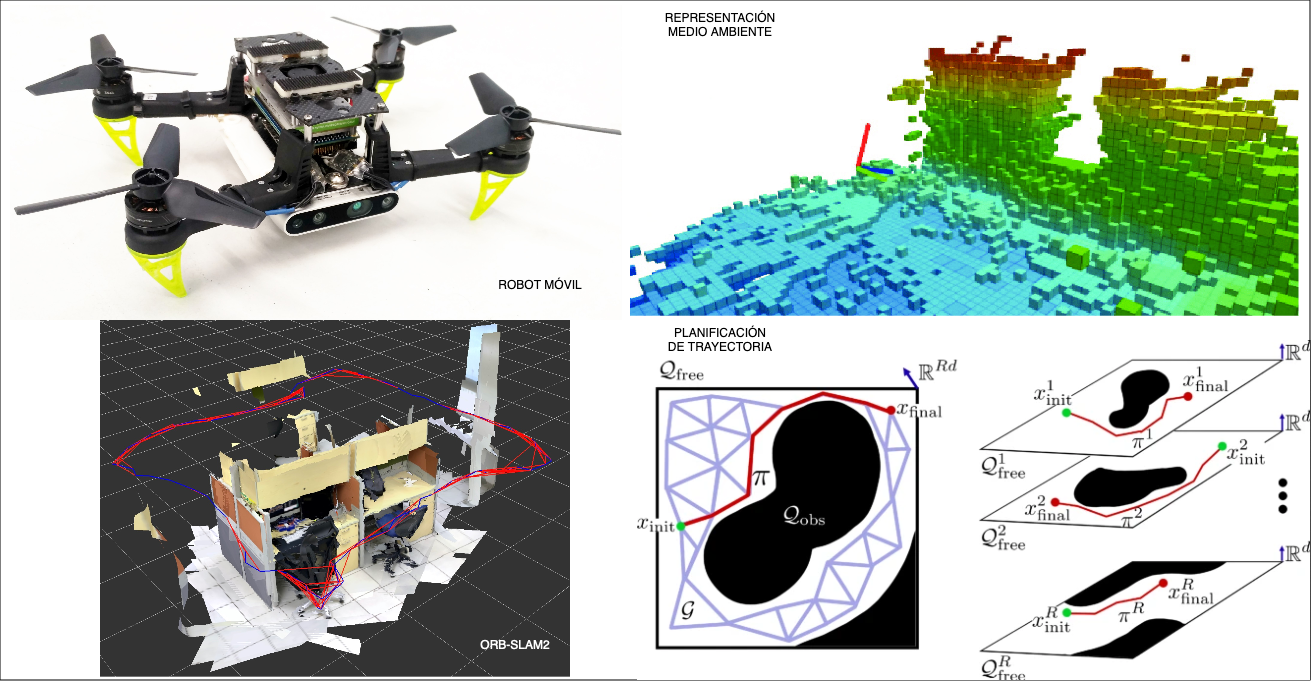
\includegraphics[width=\linewidth]{ANTECEDENTES}\\
\end{frame}

\begin{frame}{Control de un VANT \footnote{Modeling And Control Of A Quadrotor Uav With Aerodynamic Concepts, [\cite{1334249}]}}
  
  \begin{minipage}{0.47\textwidth}
     
    Estados del VANT \\
    $(x,y,z,\phi,\theta,\Psi,\dot{x},\dot{y},\dot{z},\dot{\phi},\dot{\theta},\dot{\Psi})^\mathrm{T}$

    \bigskip % Vertical whitespace
    
    Donde:
    \begin{itemize}
    \item $\xi = (x,y,z)^\mathrm{T}$ representan la posición linear
    \item $\eta = (\phi,\theta,\Psi)^\mathrm{T}$ ángulos de euler: roll, pitch, yaw
    \item $(\dot{x},\dot{y},\dot{z},\dot{\phi},\dot{\theta},\dot{\Psi})^\mathrm{T}$ velocidades lineares y angulares
    \end{itemize}
  \end{minipage}
  \hspace{0.2cm}
  \begin{minipage}{0.5\textwidth}
    \centering
    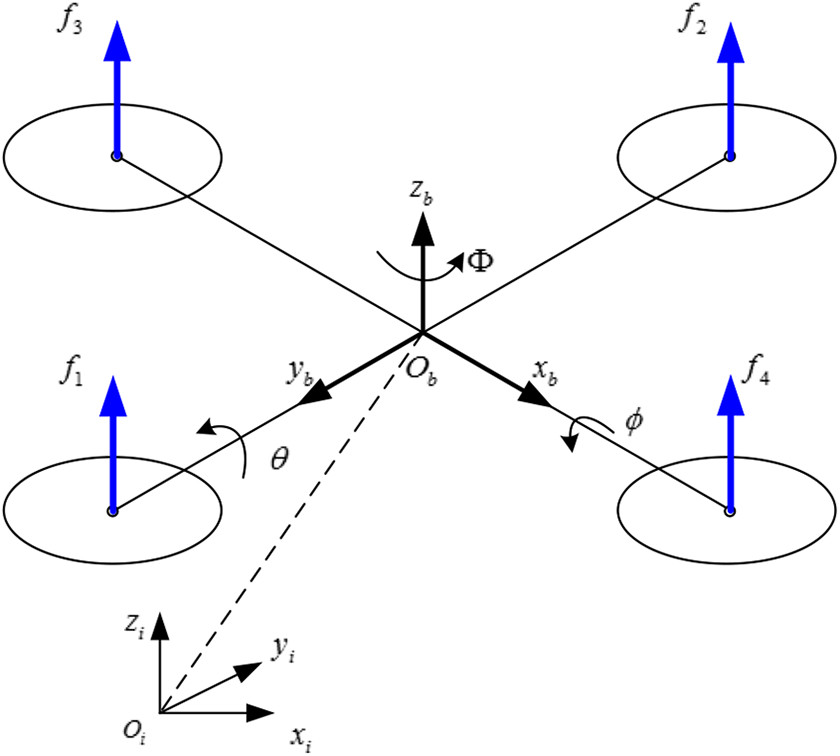
\includegraphics[width=4cm]{uav_model.jpeg}
    \bigskip % Vertical whitespace
    {\scriptsize
      \begin{itemize}
      \item Cuatro rotores.
      \item Seis grados de libertad (3 lineales y 3 angulares).
      \item Requiere cuatro variables de control $(u_1, u_2, u_3, u_4)$ para mantener su estabilidad y control durante el vuelo.
      \end{itemize}
    }
  \end{minipage}
  \bigskip % Vertical whitespace
\end{frame}

\begin{frame}{Formulación del Problema de Localización y Mapeo Simultáneos \footnote{\tiny Omni-Swarm: A Decentralized Omnidirectional Visual–Inertial–UWB State Estimation System for Aerial Swarms, [\cite{OMNI2022}]}}

  \small{
    Dados:
    \begin{itemize}
    \item Conjunto de observaciones $z(t) = \{z_1,z_2,...,z_t\}$
    \item Conjunto de comandos de control $u(t) = \{u_1,u_2,...,u_t\}$
    \end{itemize}
    %\bigskip % Vertical whitespace
    Requerimos:
    \begin{itemize}
    \item Mapa del ambiente $m$
    \item Trayectoria del robot $x(t) = \{x_1,x_2,...,x_t\}$
    \end{itemize}
    %\bigskip % Vertical whitespace
    
    En terminos probabilisticos, queremos estimar la trayectoria del robot y el mapa
  }
  \centering
  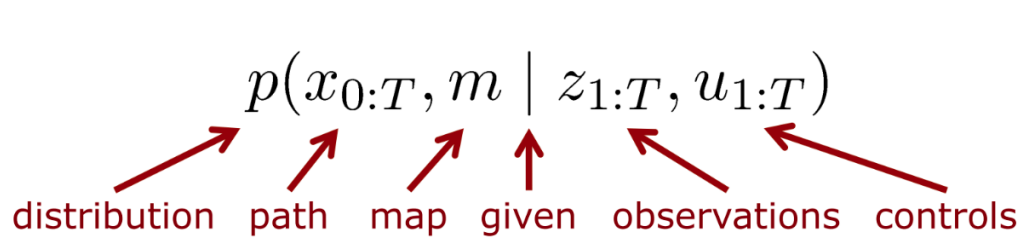
\includegraphics[width=8cm]{slam1}
  \bigskip % Vertical whitespace
\end{frame}

\begin{frame}{Formulación del Problema de Localización y Mapeo Simultáneos \footnote{\tiny Omni-Swarm: A Decentralized Omnidirectional Visual–Inertial–UWB State Estimation System for Aerial Swarms, [\cite{OMNI2022}]}}
  
  \begin{itemize}
  \item La trayectoria del robot y el mapa son desconocidos.
  \item Correlación entre el mapa y las posiciones del robot.
  \end{itemize}
  
  \centering
  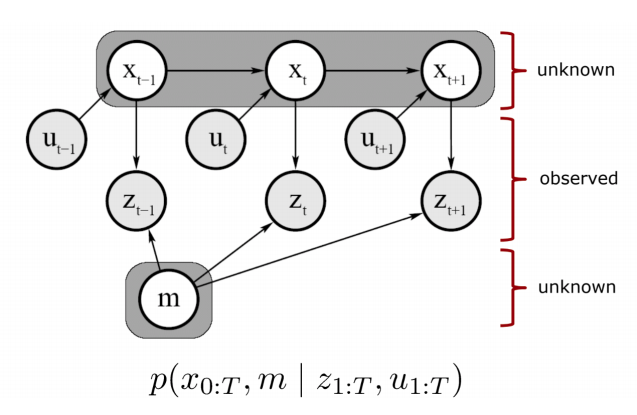
\includegraphics[width=8cm]{slam2}
  \bigskip % Vertical whitespace
\end{frame}

\begin{frame}{Representación medio ambiente \footnote{\tiny RACER: Rapid Collaborative Exploration With a Decentralized Multi-UAV System [\cite{RACER2022}]}}
  \begin{figure}[ht!]
    \centering
    \begin{minipage}{0.48\textwidth}
      \centering
      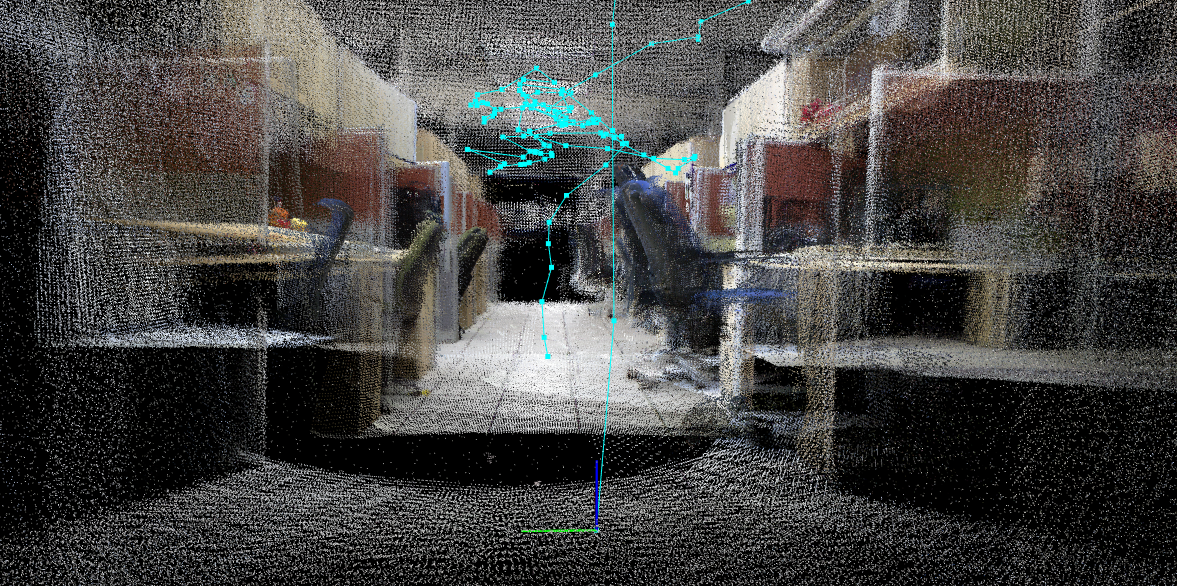
\includegraphics[width=\linewidth,height=3.5cm]{ROS_MAP2} % BUSQUEDA Y RESCATE
    \end{minipage}\hfill
    \begin{minipage}{0.48\textwidth}
      \centering
      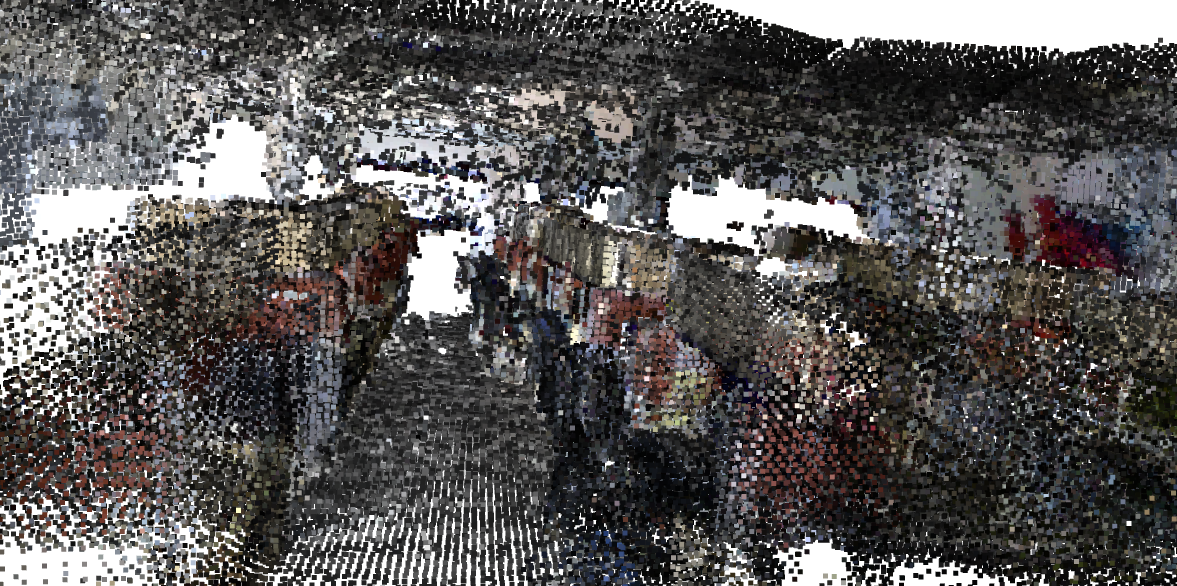
\includegraphics[width=\linewidth,height=3.5cm]{ROS_MAP3} % INSPECCION Y SEGURIDAD
    \end{minipage}
    \vspace{-0.2cm} % Espacio vertical entre imágenes
    \begin{minipage}{0.48\textwidth}
      \centering
      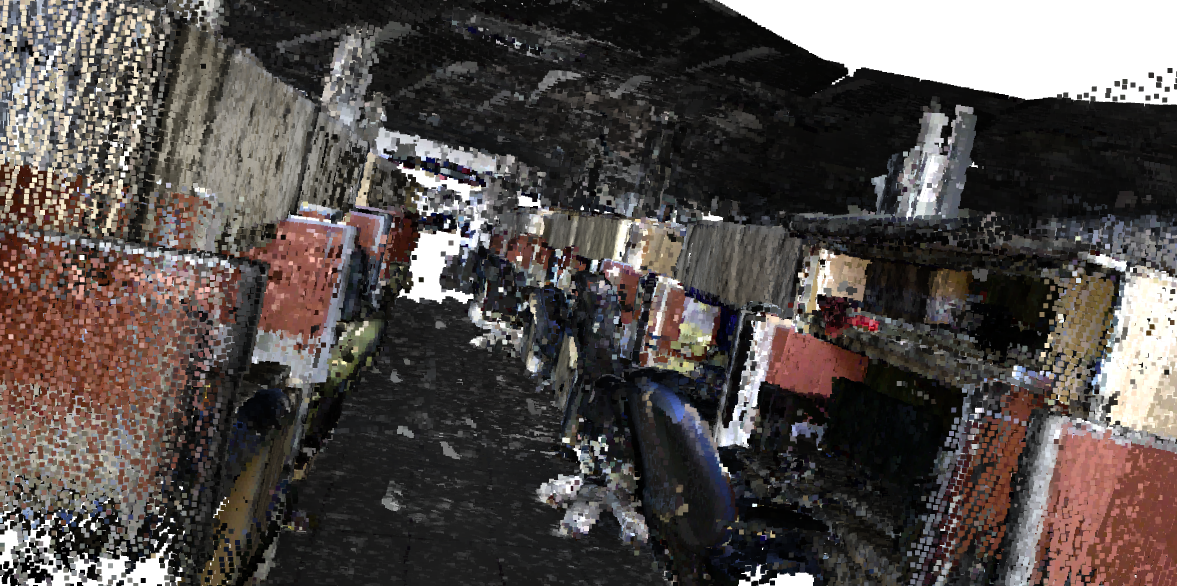
\includegraphics[width=\linewidth,height=3.5cm]{ROS_MAP4} % DRONES EN CIUDADES CON GPS DENY
    \end{minipage}\hfill
    \begin{minipage}{0.48\textwidth}
      \centering
      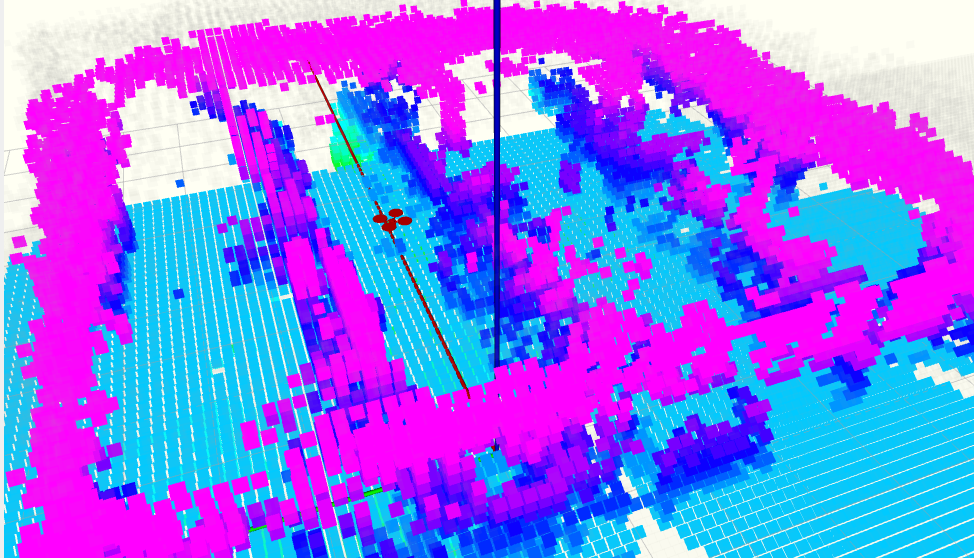
\includegraphics[width=\linewidth,height=3.5cm]{ROS_MAP6} % 
    \end{minipage}
  \end{figure}
  \bigskip % Vertical whitespace
\end{frame}

\begin{frame}{Coordinación}
  \begin{figure}[ht!]
    \centering
    \begin{minipage}{0.48\textwidth}
      {\scriptsize
      \begin{itemize}
      \item \textcolor{blue}{Descentralizada} - Cada robot es completamente independiente y planea sus propios trayectos
      \item Exploración basada en fronteras {\footnote{\tiny{A frontier-based approach for autonomous exploration [\cite{613851}]}}}
      \item Explotación, Exploración y Cohesión
      \end{itemize}
      }
    \end{minipage}\hfill
    \begin{minipage}{0.48\textwidth}
      \centering
      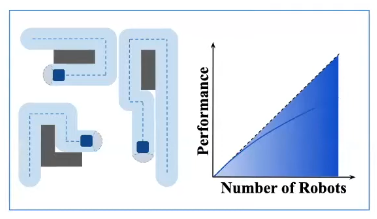
\includegraphics[width=0.6\textwidth]{coordination}{\footnote{\tiny{Beyond Robustness: A Taxonomy of Approaches towards Resilient Multi-Robot Systems [\cite{amanda}]}}}
      %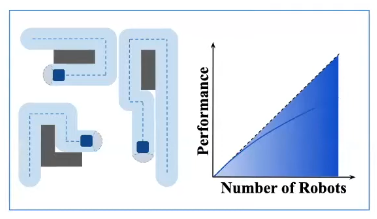
\includegraphics[width=0.8\linewidth]{coordination} % INSPECCION Y SEGURIDAD
    \end{minipage}
    \vspace{-0.2cm} % Espacio vertical entre imágenes
    \begin{minipage}{0.48\textwidth}
      {\scriptsize
      \begin{itemize}
      \item \textcolor{blue}{Problema de asignación} - Asignar tareas de exploración a los VANTs de manera que minimicen el costo total de ejecución.
      \item Para instancias mayores el algoritmo $\epsilon$ - scaling auction tiene un mayor desempeño que los otros algoritmos.{\footnote{\tiny{The assignment problem revisited [\cite{Alfaro2021}]}}}
      \end{itemize}
      }
    \end{minipage}\hfill
    \begin{minipage}{0.48\textwidth}
      \centering
      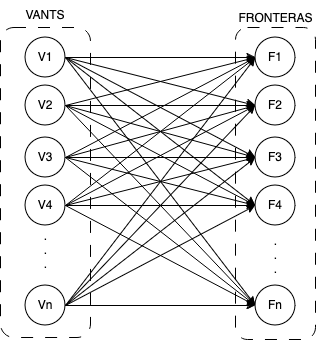
\includegraphics[width=0.5\linewidth]{asignacion} % 
    \end{minipage}
  \end{figure}
\end{frame}

\begin{frame}[fragile]{Estado del arte}
  \centering
  \scalebox{0.70}{
  \begin{tabular}{ | p{3cm} | p{1.6cm} | p{2.5cm} | p{3cm} | p{3.1cm} | p{0.8cm} | p{0.9cm} | }
    \hline    
    \tiny REFERENCIA&
    \tiny APLICACIÓN&
    \tiny GENERACION MAPA&
    \tiny PLANIFICACION DE RUTA&
    \tiny GENERACION TRAYECTORIA&
    \tiny SENSOR RGB-D&
    \tiny DINAMICA VANT\\
    \hline
    %--------------------------
    \tiny \cellcolor{gray!20}\cite{CIESLEWSKI2017}[\citenum{CIESLEWSKI2017}]&
    \tiny \cellcolor{gray!20}Exploración&
    \tiny \cellcolor{gray!20}Octomap&
    \tiny \cellcolor{gray!20}Basado en fronteras&
    \tiny \cellcolor{gray!20}Control directo de velocidad&
    \tiny \cellcolor{gray!20}\ding{51} &
    \tiny \cellcolor{gray!20}\ding{55} \\ \hline
    %--------------------------
    \tiny \cite{USENKO2017}[\citenum{USENKO2017}]&
    \tiny Punto Objetivo&
    \tiny Cuadr\'{i}cula egoc\'{e}ntrica&
    \tiny Offline RRT*&
    \tiny Curvas de Bezier&
    \tiny \ding{55} &
    \tiny \ding{51} \\ \hline
    %--------------------------
    \tiny \cite{MOHTA2017}[\citenum{MOHTA2017}]&
    \tiny Punto Objetivo&
    \tiny mapa 3D-Local y 2D-Global&
    \tiny A*&
    \tiny Programaci\'{o}n cuadr\'{a}tica&
    \tiny \ding{55} &
    \tiny \ding{51} \\ \hline
    %--------------------------
    \tiny \cite{LIN2017}[\citenum{LIN2017}]&
    \tiny Punto Objetivo&
    \tiny 3D voxel array TSDF&
    \tiny A*&
    \tiny Optimizaci\'{o}n cuadr\'{a}tica&
    \tiny \ding{55}&
    \tiny \ding{55} \\ \hline
    %--------------------------
    \tiny \cellcolor{gray!20}\cite{PAPACHRISTOS2017}[\citenum{PAPACHRISTOS2017}]&
    \tiny \cellcolor{gray!20}Exploración&
    \tiny \cellcolor{gray!20}Octomap&
    \tiny \cellcolor{gray!20}Next Best View Planner (NBVP)&
    \tiny \cellcolor{gray!20}Control directo de velocidad&
    \tiny \cellcolor{gray!20}\ding{55}&
    \tiny \cellcolor{gray!20}\ding{55} \\ \hline
    %--------------------------
    \tiny \cite{OLEYNIKOVA2018}[\citenum{OLEYNIKOVA2018}]&
    \tiny Punto Objetivo&
    \tiny Voxel Hashing TSDF&
    \tiny Next Best View Planner (NBVP)&
    \tiny Optimizaci\'{o}n cuadr\'{a}tica&
    \tiny \ding{51}&
    \tiny \ding{51} \\ \hline
    %--------------------------
    \tiny \cite{GAO2018}[\citenum{GAO2018}]&
    \tiny Punto Objetivo&
    \tiny Mapa de cuadr\'{i}cula&
    \tiny M\'{e}todo de marcha r\'{a}pida&
    \tiny Optimizaci\'{o}n cuadr\'{a}tica&
    \tiny \ding{55}&
    \tiny \ding{51} \\ \hline
    %--------------------------
    \tiny \cite{FLORENCE2018}[\citenum{FLORENCE2018}]&
    \tiny Punto Objetivo&
    \tiny Busqueda basada en visibilidad&
    \tiny 2D A*&
    \tiny Control predictivo por modelo (MPC)&
    \tiny \ding{51}&
    \tiny \ding{51} \\ \hline
    %--------------------------
    \tiny \cellcolor{gray!20}\cite{SELIN2019}[\citenum{SELIN2019}]&
    \tiny \cellcolor{gray!20}Exploración&
    \tiny \cellcolor{gray!20}Octomap&
    \tiny \cellcolor{gray!20}Next Best View Planner (NBVP)&
    \tiny \cellcolor{gray!20}Control directo de velocidad&
    \tiny \cellcolor{gray!20}\ding{55}&
    \tiny \cellcolor{gray!20}\ding{55} \\ \hline
    %--------------------------
    \tiny \cellcolor{gray!20}\cite{BUG2019}[\citenum{BUG2019}]&
    \tiny \cellcolor{gray!20}Exploración&
    \tiny \cellcolor{gray!20}NA&
    \tiny \cellcolor{gray!20}Swarm Gradient Bug Algorithm (SGBA)&
    \tiny \cellcolor{gray!20}Control directo de velocidad&
    \tiny \cellcolor{gray!20}\ding{55}&
    \tiny \cellcolor{gray!20}\ding{55} \\ \hline
    %--------------------------
    \tiny \cite{COLLINS2019}[\citenum{COLLINS2019}]&
    \tiny Punto Objetivo&
    \tiny KD Tree $+$ Mapa en Voxel&
    \tiny B\'{u}squeda en Grafo&
    \tiny Movimientos suaves&
    \tiny \ding{51}&
    \tiny \ding{51} \\ \hline
    %--------------------------
    \tiny \cite{CINVES2021}[\citenum{CINVES2021}]&
    \tiny Punto Objetivo&
    \tiny Octree&
    \tiny Rapidly Exploring Random Trees (RRT)&
    \tiny Basado en contornos&
    \tiny \ding{51}&
    \tiny \ding{51} \\ \hline
    %--------------------------
    \tiny \cellcolor{gray!20}\cite{CIESLEWSKI2021}[\citenum{CIESLEWSKI2021}]&
    \tiny \cellcolor{gray!20}Exploración&
    \tiny \cellcolor{gray!20}Octomap&
    \tiny \cellcolor{gray!20}Basado en fronteras&
    \tiny \cellcolor{gray!20}Control directo de velocidad&
    \tiny \cellcolor{gray!20}\ding{51}&
    \tiny \cellcolor{gray!20}\ding{55} \\ \hline
    %--------------------------
    \tiny \cellcolor{gray!20}\cite{RACER2022}[\citenum{RACER2022}]&
    \tiny \cellcolor{gray!20}Exploración&
    \tiny \cellcolor{gray!20}HGrid&
    \tiny \cellcolor{gray!20}Next Best View Planner (NBVP)&
    \tiny \cellcolor{gray!20}Control directo de velocidad&
    \tiny \cellcolor{gray!20}\ding{51}&
    \tiny \cellcolor{gray!20}\ding{51} \\ \hline
    %--------------------------
    %\scriptsize \cite{WESTHEIDER2023}[\citenum{WESTHEIDER2023}]&
    %\scriptsize Mapa de cuadrícula&
    %\scriptsize Deep Reinforcement Learning&
    %\scriptsize Control directo de velocidad \\ \hline
    %--------------------------
    \tiny \cellcolor{gray!20}\cite{BARTOLOMEI2023}[\citenum{BARTOLOMEI2023}]&
    \tiny \cellcolor{gray!20}Exploración&
    \tiny \cellcolor{gray!20}HGrid&
    \tiny \cellcolor{gray!20}Basado en fronteras&
    \tiny \cellcolor{gray!20}Control directo de velocidad&
    \tiny \cellcolor{gray!20}\ding{51}&
    \tiny \cellcolor{gray!20}\ding{51} \\ \hline
    %--------------------------
  \end{tabular}
  }
\end{frame}

\begin{frame}{Planificación trayectoria}
  \centering
  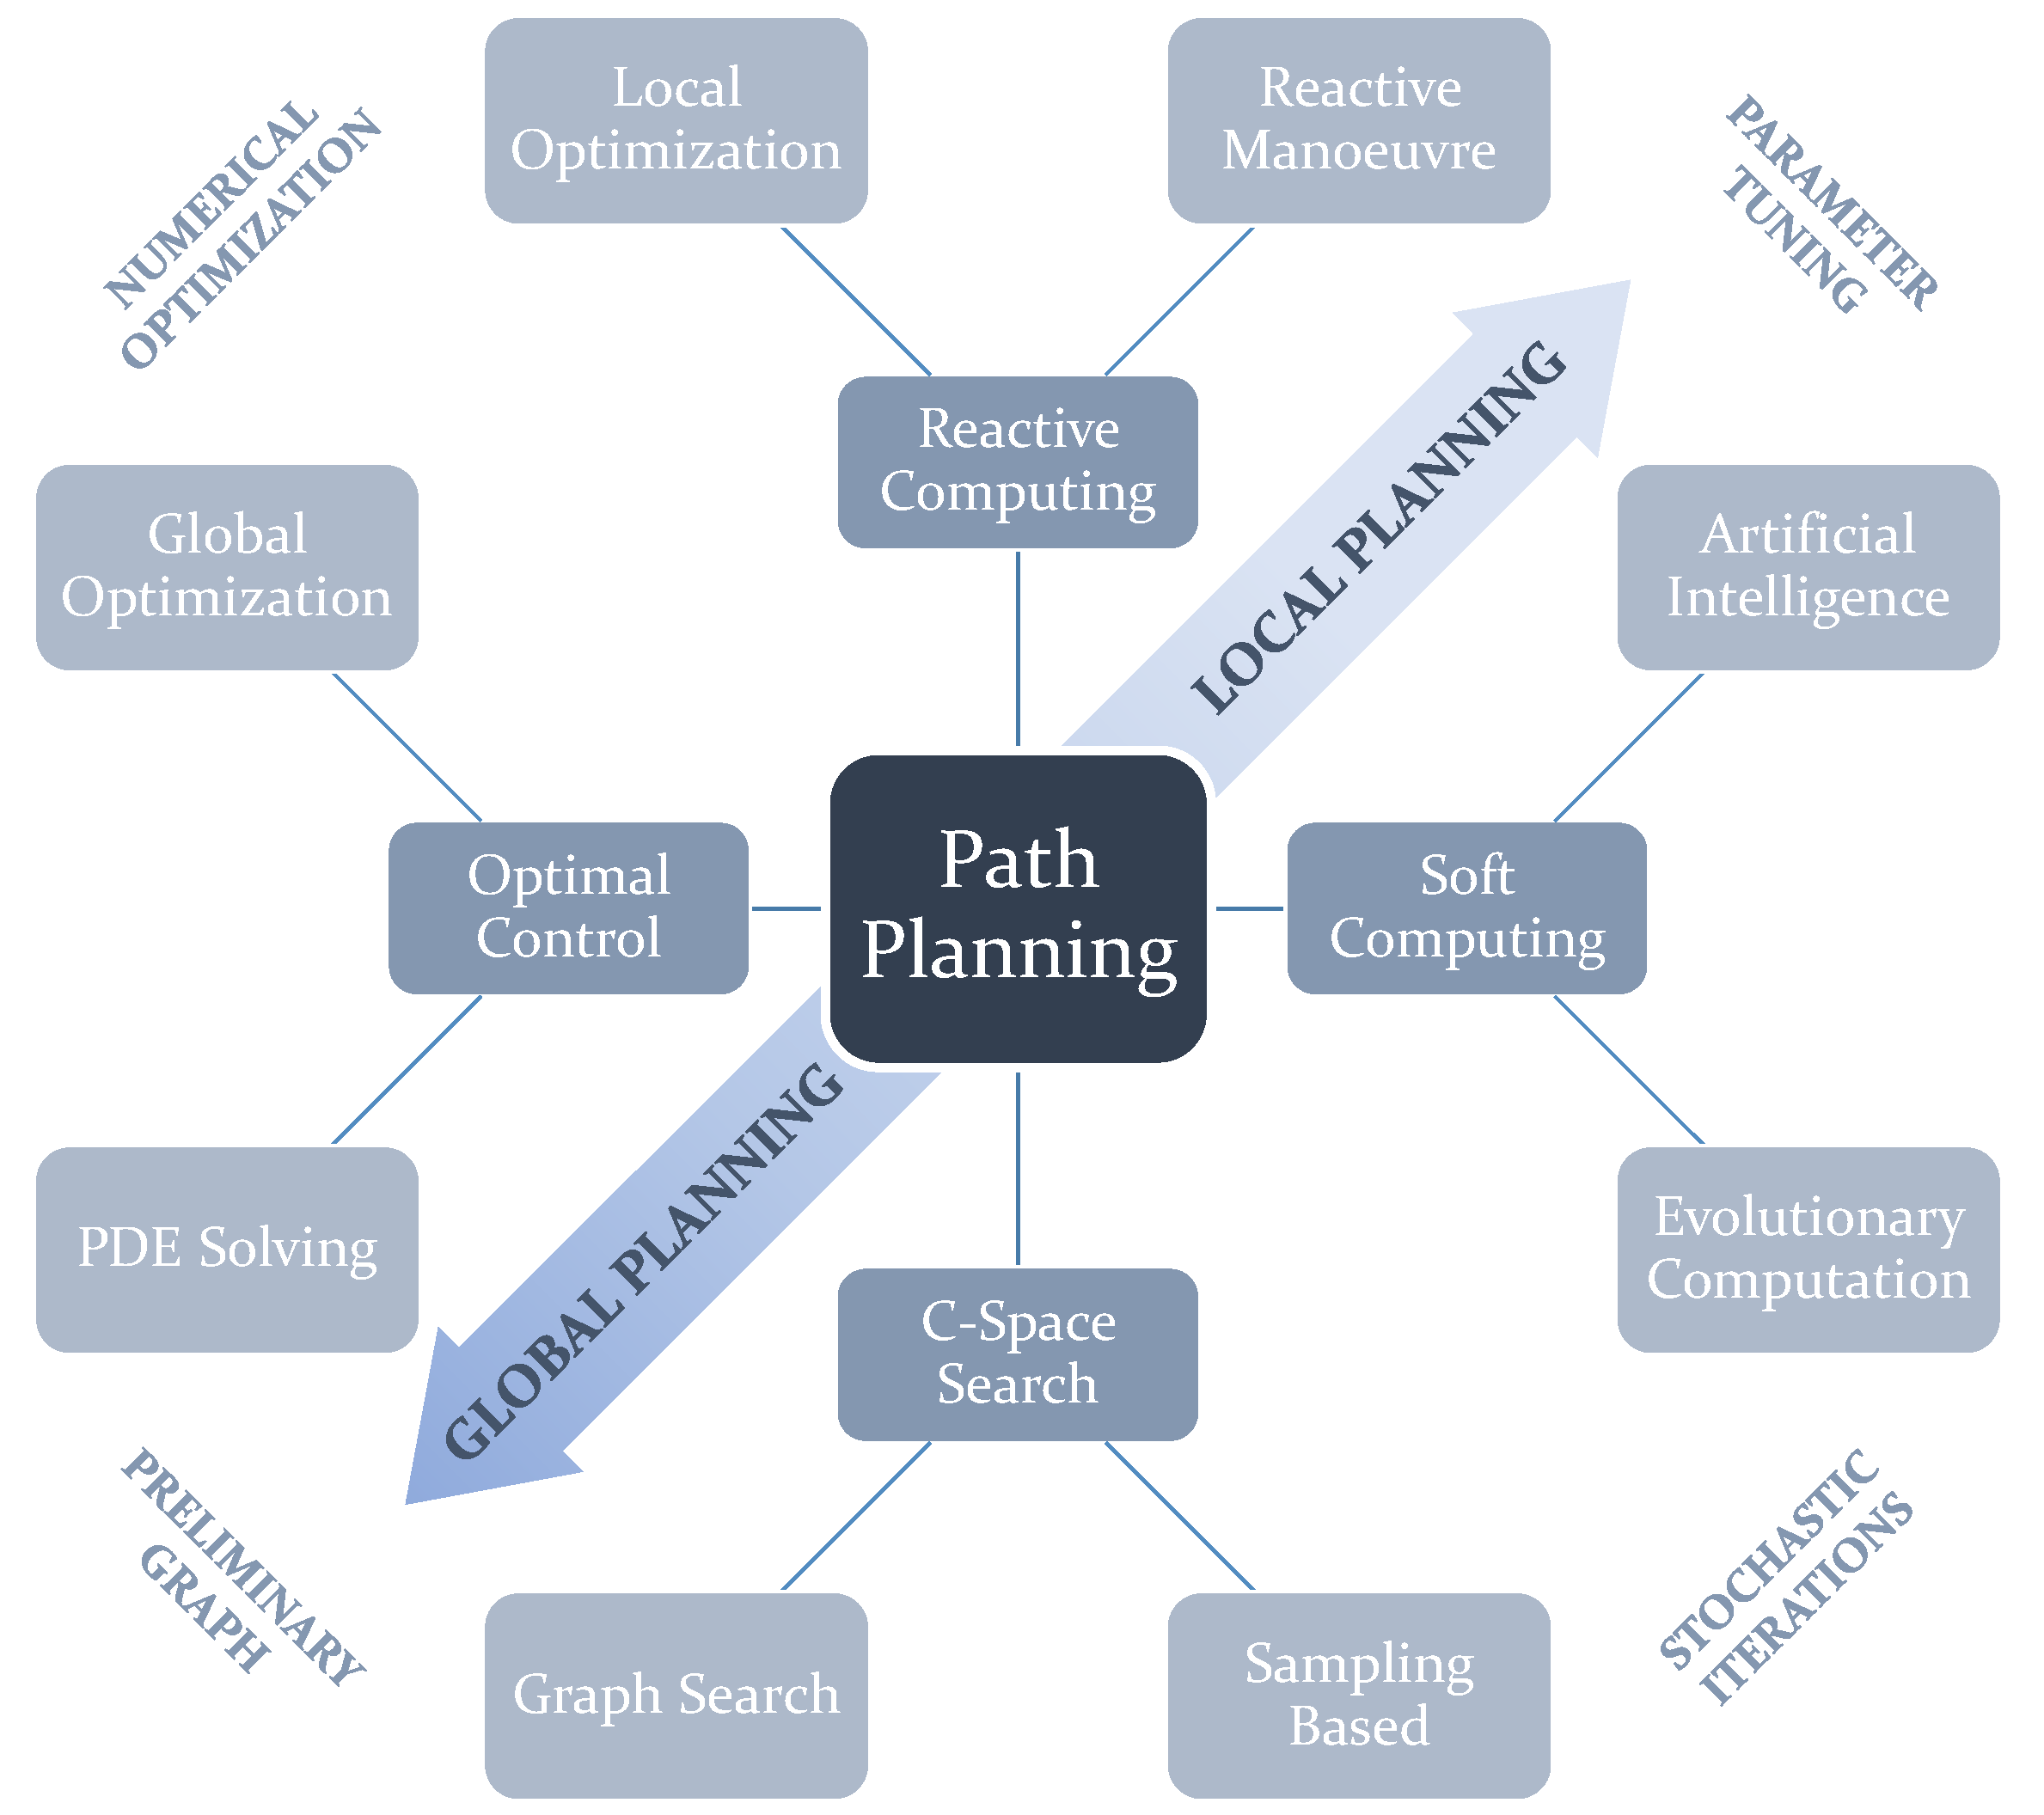
\includegraphics[width=10cm, height=6cm]{panorama_planning}
\end{frame}

\begin{frame}[allowframebreaks,noframenumbering]
  \tiny
  \bibliographystyle{abbrvnat}
  \bibliography{demo}
\end{frame}

\end{document}
